\chapter{Xarxa Neuronal}
\section{Introducció}\label{sec:intr}
En iniciar la part pràctica del treball vam decidir crear tres tipus de xarxes neuronals: una \nameref{sec:10}, una altra \nameref{sec:11} i, finalment, una \nameref{sec:12}.

En aquest capítol explicarem com vam elaborar cadascuna d’aquestes xarxes neuronals i, a més, compararem les dues formes de desenvolupament en una \nameref{sec:op}.

Per facilitar l’organització del treball, ens hem repartit les tasques: un membre de l’equip s’ha encarregat de la xarxa neuronal implementada amb llenguatge de programació Python, mentre que l’altre ha treballat una xarxa neuronal feta amb fulls de càlcul. Finalment, hem elaborat conjuntament la taula de comparació, intercanviant perspectives, i també hem treballat plegats la xarxa neuronal del cas real.

Les nostres pràctiques consisteixen en recopilar una sèrie de dades d'alumnes mitjançant una enquesta feta per nosaltres amb la finalitat de crear una Xarxa neuronal que pugues predir la nota final de cada alumne. Les preguntes fetes en el formulari són sobre la matèria de matemàtiques i són les següents:
\begin{itemize}
 \item Realització de deures
 \item Hores d'estudis (semanal)
 \item Hores de section
 \item Interès en la matèria
 \item Nota del segon trimestre
 \item Nota del tercer trimestre
 \item Nota final
\end{itemize}
Com es pot veure, les preguntes d'aquest formulari estan relacionades amb el rendiment d'estudis dels alumnes, i s'envia als estudiants que tingues l'assignatura matematiques.

Mostra del formulari:
\begin{figure}[H]
    \centering
    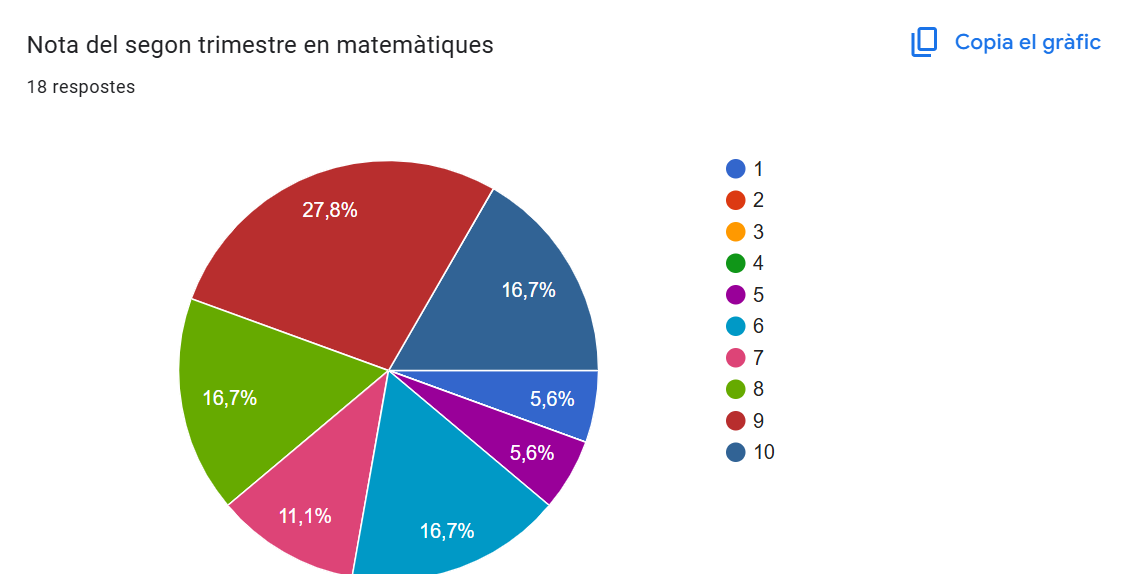
\includegraphics[width=0.5\textwidth]{./figures/14.png}
    \caption{Nota del segon trimestre}
\end{figure}

\begin{figure}[H]
    \centering
    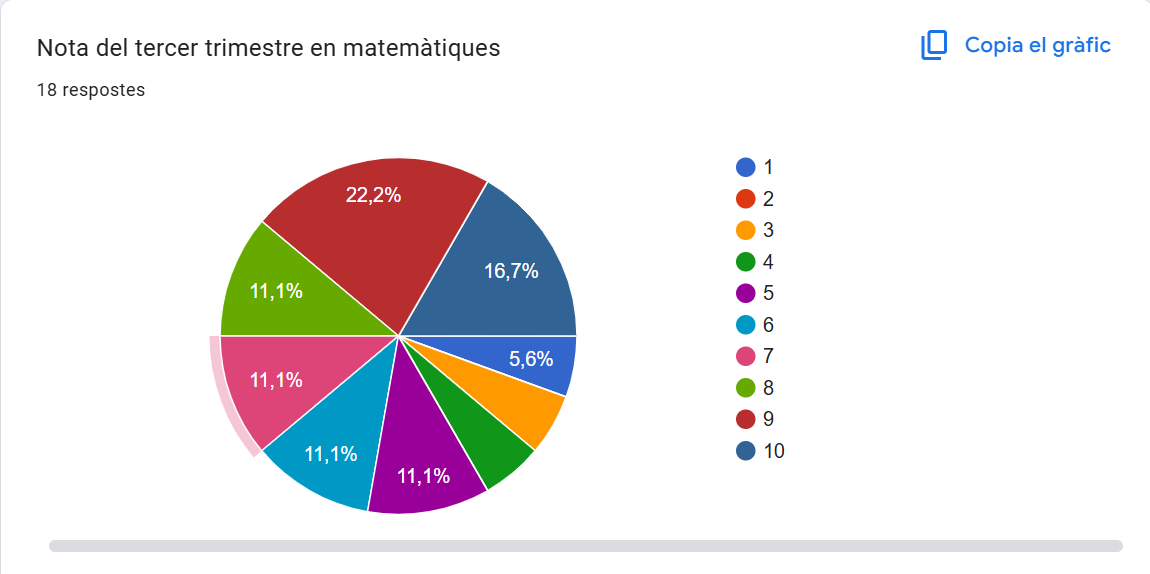
\includegraphics[width=0.5\textwidth]{./figures/15.png}
    \caption{Nota del tercer trimestre}
\end{figure}

\begin{figure}[H]
    \centering
    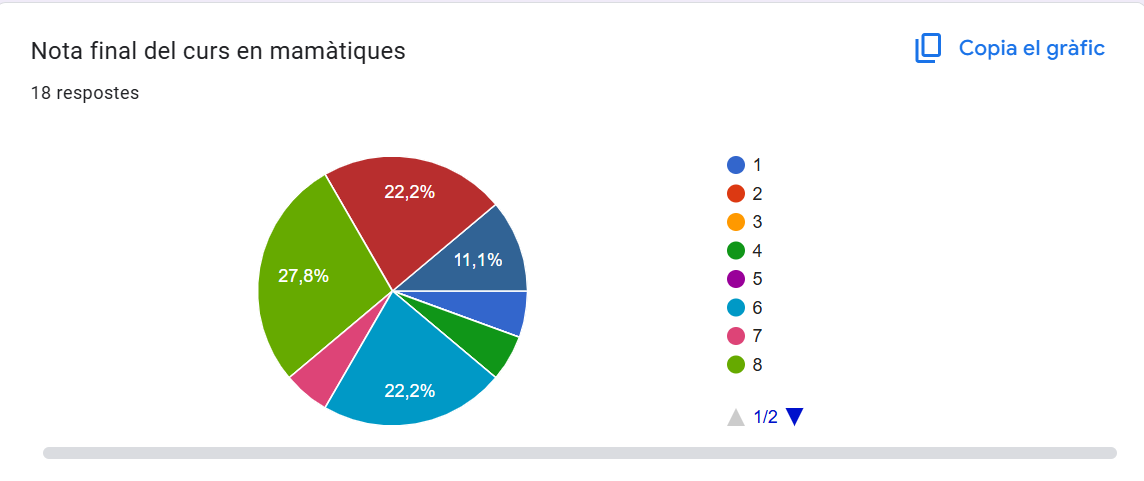
\includegraphics[width=0.5\textwidth]{./figures/16.png}
    \caption{Nota final del curs}
\end{figure}

\begin{figure}[H]
    \centering
    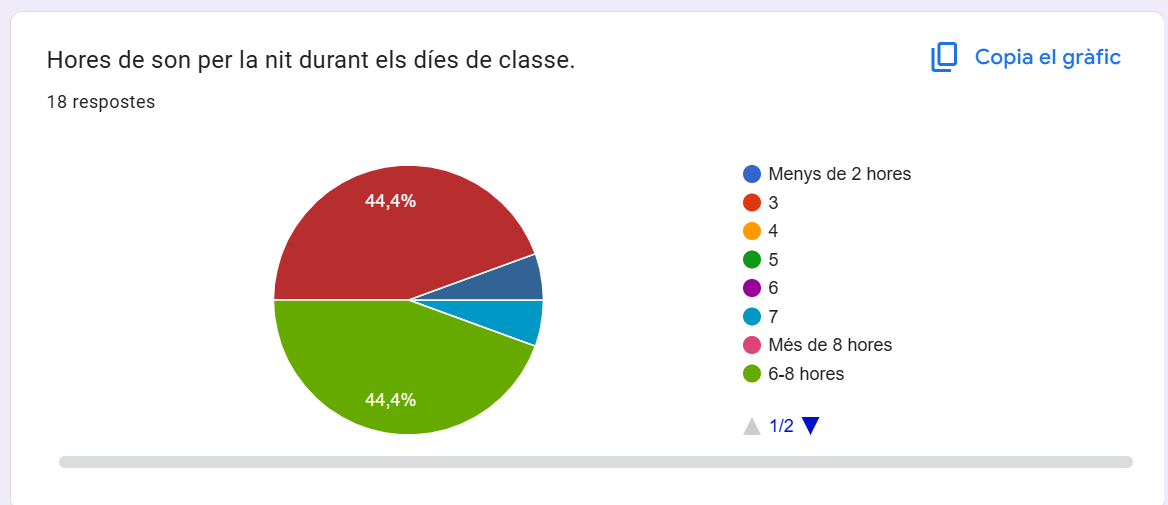
\includegraphics[width=0.5\textwidth]{./figures/17.png}
    \caption{Hores de son per la nit durant l'horari escolar}
\end{figure}

\begin{figure}[H]
    \centering
    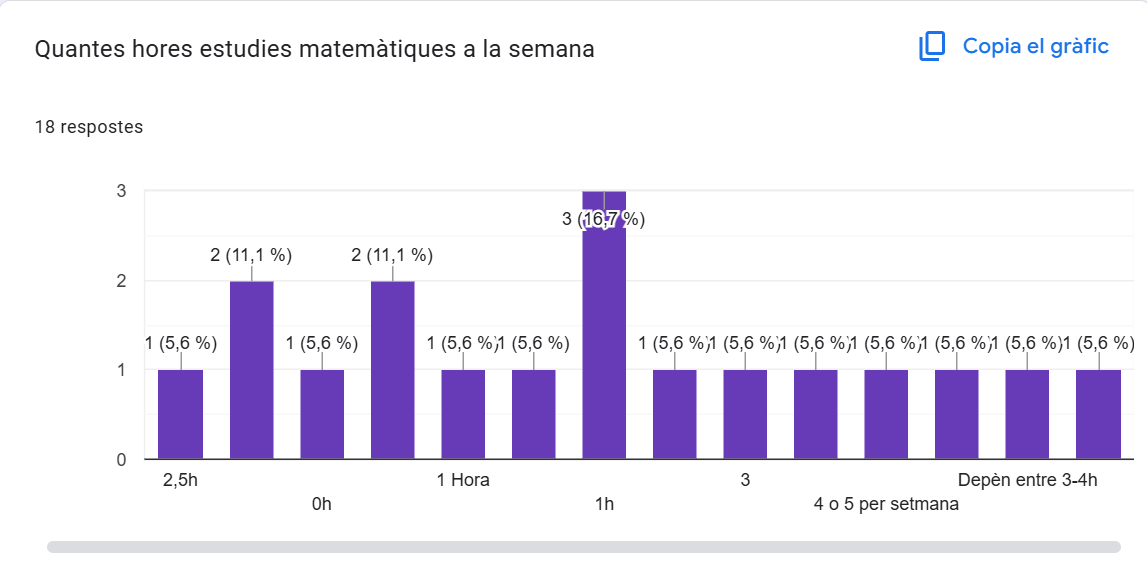
\includegraphics[width=0.5\textwidth]{./figures/18.png}
    \caption{Cuantes hores estudies a la semana}
\end{figure}

\begin{figure}[H]
    \centering
    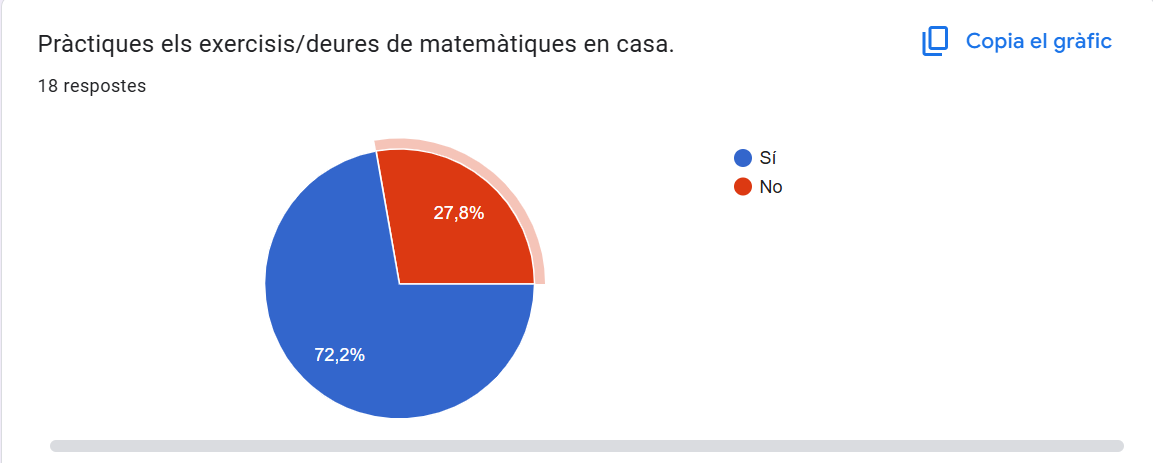
\includegraphics[width=0.5\textwidth]{./figures/19.png}
    \caption{Pràctiques a casa}
\end{figure}

\begin{figure}[H]
    \centering
    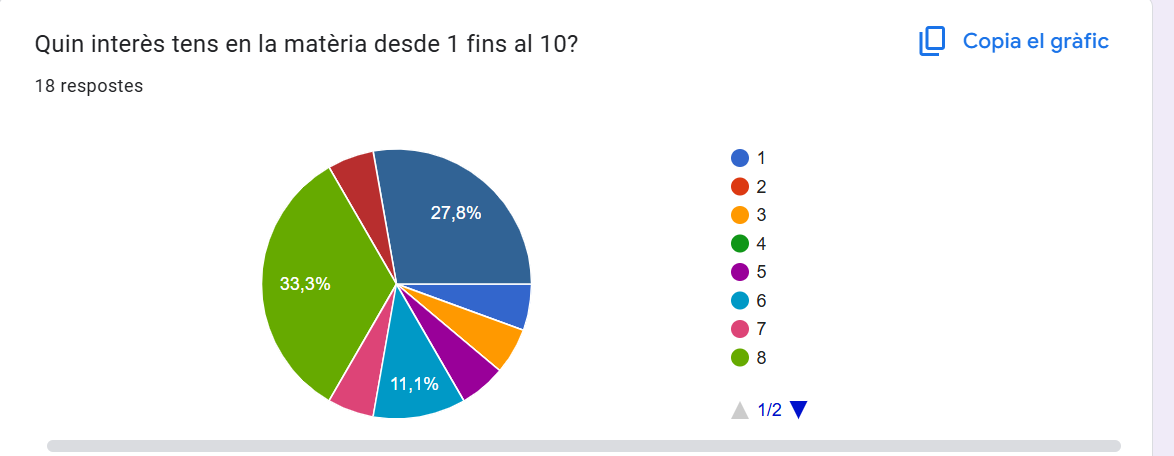
\includegraphics[width=0.5\textwidth]{./figures/20.png}
    \caption{Interès cap a l'assignatura}
\end{figure}



Després de les prediccions, compararem la xarxa neuronal feta amb python y la del full de càlcul i veurem quina de les dos té més precisió.

\section{Xarxa neuronal de regressió}\label{sec:op}
Una intel·ligència artificial és un camp molt extens i, dins d’aquest, les xarxes neuronals també representen una branca àmplia i complexa.
En el nostre context utilitzarem un tipus concret de xarxa neuronal per a la pràctica: les \textbf{xarxes neuronals de regressió}.

Una xarxa neuronal de regressió, a diferència d’una de classificació, té una sortida de tipus lineal que permet predir un valor numèric continu. Aquest tipus de xarxes requereixen un conjunt de dades prou extens i ben estructurat per poder aprendre les relacions entre les variables d’entrada i generar una estimació fiable.

A continuació es mostra un esquema representatiu d’una xarxa neuronal de regressió:

\begin{figure}[h!]
\centering
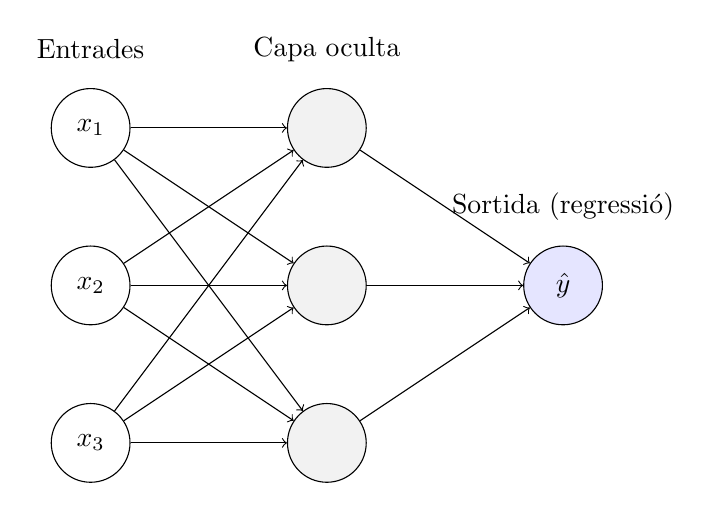
\begin{tikzpicture}[scale=1, transform shape]

% Input layer
\node[circle, draw, minimum size=1cm] (I1) at (0,2) {$x_1$};
\node[circle, draw, minimum size=1cm] (I2) at (0,0) {$x_2$};
\node[circle, draw, minimum size=1cm] (I3) at (0,-2) {$x_3$};

% Hidden layer
\node[circle, draw, fill=gray!10, minimum size=1cm] (H1) at (3,2) {};
\node[circle, draw, fill=gray!10, minimum size=1cm] (H2) at (3,0) {};
\node[circle, draw, fill=gray!10, minimum size=1cm] (H3) at (3,-2) {};

% Output layer
\node[circle, draw, fill=blue!10, minimum size=1cm] (O1) at (6,0) {$\hat{y}$};

% Connections input -> hidden
\foreach \i in {1,2,3}
  \foreach \h in {1,2,3}
    \draw[->] (I\i) -- (H\h);

% Connections hidden -> output
\foreach \h in {1,2,3}
  \draw[->] (H\h) -- (O1);

% Labels
\node at (0,3) {Entrades};
\node at (3,3) {Capa oculta};
\node at (6,1) {Sortida (regressió)};

\end{tikzpicture}
\caption{Esquema d’una xarxa neuronal de regressió}
\end{figure}

\section{Xarxa Neuronal amb llenguatge de programació}\label{sec:10}
En aquest apartat explicarem pas a pas de com vaig crear el nostre xarxa neuronal de regressió amb un llenguatge de programació.

\subsection{De celcius a fahrenheit}

Abans de començar a treballar amb la xarxa neuronal definitiu, vaig voler fer una de més simple per tal de coneixer amb més profunditat de com funciona una xarxa neuronal de regressió; en aquest cas he escollit un transformador d'unitats de temperatura, de celcius (\textbf{Unitat de temperatura basada en el punt de fusió de l'aigua}) a fahrenheit (\textbf{Sistema d'unitat basada en el punt d'ebullició i solidificació de l'aigua}). Per crear aquesta xarxa vaig escollir el Python com a llenguatge de programació, i el motiu esta explicat en l'apartat \ref{sec:4.4}.\\


Per començar, importo el framework i la biblioteca de Python que són les bases de dades necessàries per a la creació de la xarxa neuronal: \texttt{TensorFlow} (\textbf{framework}) i \texttt{{numpy}} (\textbf{biblioteca}). Com podeu veure, he creat uns \textit{abrevacions} per a poder-los cridar més fàcilment quan els necessiti.

\begin{itemize}
 \item \textbf{TensorFlow: }\label{TensorFlow} TensorFlow és un tipus de framework en que ofereix eines per crear i entrenar models de Ml (Machine learning) i Dl (Deep learning), biblioteques per programar xarxes neuronals i altres algoritmes, Compatibilitat amb GPU i TPU per accelerar càlculs, TensorBoard per visualitzar i monitorar entrenaments, Models preentrenats i repositoris, APIs (Application Programming Interface) en diversos llenguatges.
 \item \textbf{numpy: }\label{numpy} numpy és una biblioteca científica per treballar amb vectors i matrius.
\end{itemize}
\begin{figure}[H]
    \centering
    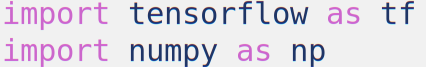
\includegraphics[width=0.5\textwidth]{./figures/1.png}
    \caption{Framework i biblioteca del Python}
\end{figure}


Agafo les paraules \textbf{celsius} i \textbf{fahrenheit} i les defineixo com a variables amb un signe \texttt{=}. Després poso \texttt{np} per indicar la biblioteca, seguit de \texttt{.array()} per especificar que és una llista. Dins dels parèntesis hi poso \texttt{[ ]} i a dins, els diferents valors de temperatura. Finalment, afegeixo el paràmetre \texttt{dtype=float} per indicar que es tracta de dades numèriques decimals.

Repeteixo el mateix procés amb \textbf{fahrenheit}, però en aquest cas les dades no poden ser arbitràries, sinó que han de ser les temperatures corresponents a les de \textbf{celsius} convertides a Fahrenheit. D’aquesta manera, la xarxa neuronal pot entendre la relació entre les dues sèries de dades.


\begin{figure}[H]
    \centering
    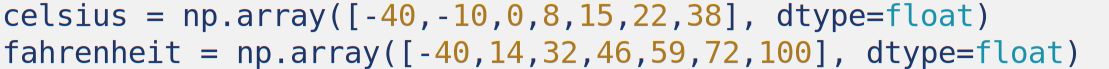
\includegraphics[width=0.5\textwidth]{./figures/2.png}
    \caption{Agrupació de dades amb numpy}
\end{figure}

Per començar, defineixo les capes de la xarxa neuronal. Utilitzant \texttt{tf.keras.layers.Dense} (\textbf{funció per a capes denses} (Keras és un tipus de API)), creo la primera capa oculta amb el paràmetre \texttt{units=3} per especificar que tingui \textbf{3 neurones}, i \texttt{input\_shape=[1]} per indicar que l'entrada és un sol valor. Li assigno el nom \texttt{oculte\_1}.\\ \\
Repeteixo el procés per a la segona capa oculta, \texttt{oculte\_2}, amb \texttt{units=3} neurones també, però sense especificar \texttt{input\_shape} ja que la xarxa ho dedueix automàticament de la capa anterior.\\ \\
Finalment, defineixo la capa de \texttt{sortida} amb \texttt{units=1} perquè retorni un sol valor (la predicció en Fahrenheit).\\ \\
Amb totes les capes creades, les integro en un model seqüencial amb \texttt{tf.keras.Sequential}, passant-les dins d'una llista \texttt{[ ]} en l'ordre correcte: \texttt{[oculte\_1, oculte\_2, sortida]}. Això crea l'estructura bàsica de la nostra xarxa neuronal.


\begin{figure}[H]
    \centering
    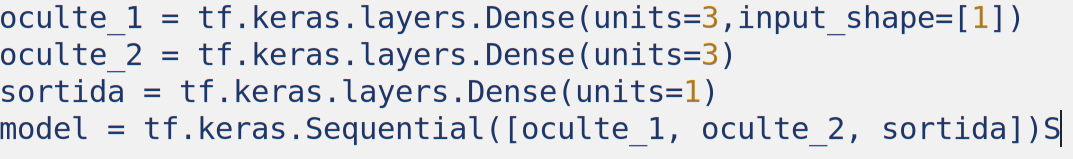
\includegraphics[width=0.5\textwidth]{./figures/3.png}
    \caption{Capes ocultes i la sortida d'una xarxa neuronal}
\end{figure}


Després de dissenyar l’estructura de la xarxa neuronal, cal ensenyar al model com aprendre i entrenar-se.
Per fer-ho utilitzem la variable \textbf{model}, a la qual ja havíem assignat les capes ocultes i la capa de sortida.
Tot seguit afegim la instrucció \textbf{.compile()}, que serveix per configurar el model abans de començar l’entrenament.

Dins de \texttt{.compile()} especifiquem el paràmetre \textbf{optimizer}, que indica la manera com el model ajustarà els pesos.
En aquest cas utilitzem \texttt{"adam"}, un optimitzador adaptatiu que redueix la velocitat d’aprenentatge quan detecta canvis bruscos en un pes,
l’augmenta quan el pes és estable i, alhora, recorda la direcció correcta per evitar oscil·lacions innecessàries.

A continuació, definim la funció de pèrdua amb el paràmetre \textbf{loss=\texttt{"mean\_squared\_error"}}.
La funció de pèrdua (\textit{loss}) mesura l’error del model i guia el procés d’aprenentatge.
En aquest cas, l’opció \texttt{mean squared error} (MSE, error quadràtic mitjà) és especialment útil en problemes de regressió,
ja que penalitza més fortament els errors grans i permet aconseguir prediccions més precises.


\begin{figure}[H]
    \centering
    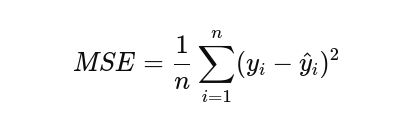
\includegraphics[width=0.5\textwidth]{./figures/5.png}
    \caption{Funció de pèrdua}
\end{figure}


\begin{figure}[H]
    \centering
    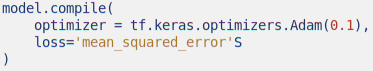
\includegraphics[width=0.5\textwidth]{./figures/4.png}
    \caption{Optimizació de la xarxa neuronal}
\end{figure}

Ara cal incloure la part crucial d'una xarxa neuronal: l'entrenament. Per fer-ho, utilitzem la variable \texttt{historial} per guardar l'evolució de l'entrenament i el model definit, \texttt{model}, aplicant-li el mètode \texttt{.fit()} que es el atribut que indica entrenament. Dins \texttt{.fit()} especifiquem, en ordre, les dades d'entrada (\texttt{celcius}), les dades de sortida (\texttt{fahrenheit}), el nombre de vegades que s'entrenarà la xarxa (\texttt{epochs=100}) i si volem mostrar el procés per pantalla (\texttt{verbose=1}, on 1 significa que sí i 0 que no).

A més, podem utilitzar \texttt{print()} per escriure comentaris o textos al terminal; en aquest cas hem posat \texttt{"Començem a entrenar..."} abans de començar i \texttt{"Model entrenat!"} un cop finalitzat l'entrenament.

\begin{figure}[H]
    \centering
    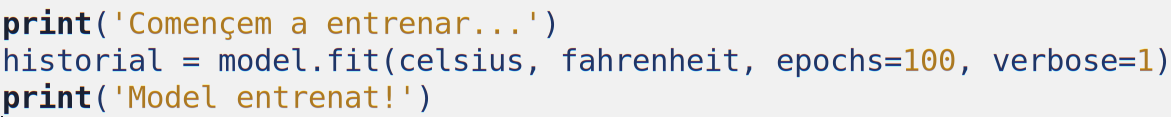
\includegraphics[width=0.5\textwidth]{./figures/6.png}
    \caption{L'entrenament de la xarxa neuronal}
\end{figure}
\label{matplotlib}
Després d’haver entrenat la xarxa neuronal i emmagatzemat l’evolució de la pèrdua a la variable \texttt{historial}, podem visualitzar com ha canviat la pèrdua a cada època utilitzant \texttt{matplotlib.pyplot}, una biblioteca de Python per crear gràfiques.

Primer, importem la biblioteca amb \texttt{import matplotlib.pyplot as plt}. A continuació, etiquetem els eixos de la gràfica amb \texttt{plt.xlabel("\# Època")} i \texttt{plt.ylabel("Magnitud de pèrdua")} per indicar què representa cada eix.

Per dibuixar la corba de la pèrdua utilitzem \texttt{plt.plot(historial.history[``loss''])}, que accedeix a la llista de valors de pèrdua que Keras ha guardat per cada època durant l’entrenament. Finalment, amb \texttt{plt.show()} mostrem la gràfica en una finestra del terminal o del notebook.

D’aquesta manera podem observar visualment si el model aprèn correctament, com disminueix la pèrdua al llarg de les èpoques i si hi ha comportaments irregulars que requeririen ajustar els paràmetres d’entrenament.

\begin{figure}[H]
    \centering
    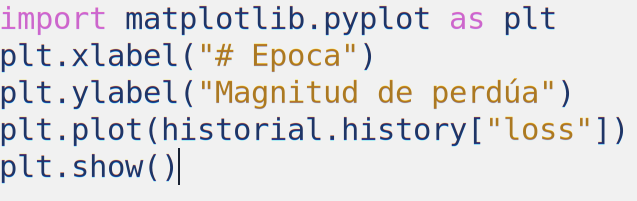
\includegraphics[width=0.5\textwidth]{./figures/7.png}
    \caption{La corba de pèrdua}
\end{figure}

Després d’haver entrenat la xarxa neuronal, podem fer prediccions amb nous valors d’entrada. Primer, utilitzem \texttt{print("Fem una predicció!")} per mostrar un missatge al terminal indicant que comença la predicció.

A continuació, fem servir \texttt{model.predict()} per calcular la predicció de la xarxa neuronal. En aquest cas, introduïm un valor de 100 graus Celsius amb \texttt{np.array([[100.0]], dtype=float)}, assegurant-nos que sigui un valor numèric decimal. El resultat s’emmagatzema a la variable \texttt{resultat}.

Finalment, utilitzem \texttt{print("El resultat es " + str(resultat) + " fahrenheit")} per mostrar la predicció obtinguda en Fahrenheit(el str es perque el variable resultat no sigui numeric sino un text). D’aquesta manera podem veure com el model converteix qualsevol temperatura de Celsius a Fahrenheit després de l’entrenament.


\begin{figure}[H]
    \centering
    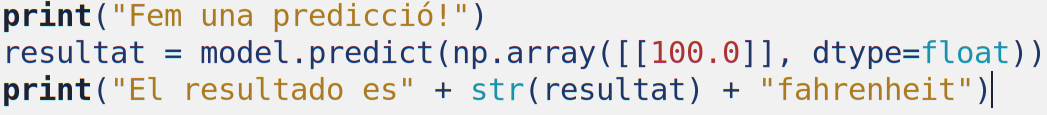
\includegraphics[width=0.5\textwidth]{./figures/8.png}
    \caption{Resultat de la predicció}
\end{figure}

Per a inspeccionar els pesos interns de la xarxa neuronal, podem utilitzar el mètode \texttt{.get\_weights()} en cada capa. Si el posem en els variables que haviem assignat les capes, per exemple, \texttt{oculte\_1.get\_weights()}, \texttt{oculte\_2.get\_weights()} i \texttt{sortida.get\_weights()} permeten veure els valors dels pesos i els biaixos que el model ha après durant l’entrenament, mostrant-los amb \texttt{print()}.


\begin{figure}[H]
    \centering
    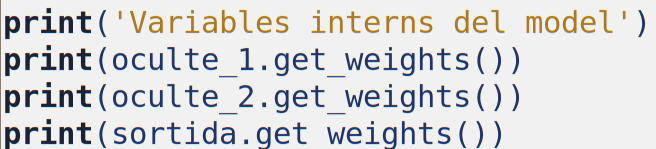
\includegraphics[width=0.5\textwidth]{./figures/9.png}
    \caption{Els pesos i biaixos assignats}
\end{figure}

Aquí hi és una mostra del resultat que dona:

\begin{figure}[H]
    \centering
    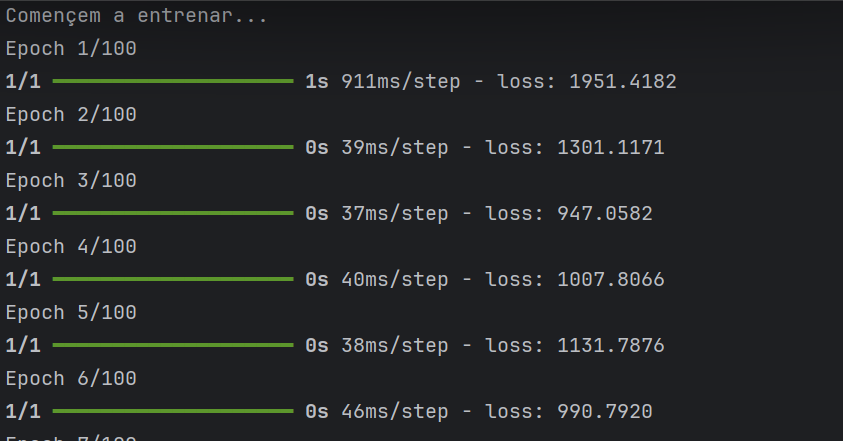
\includegraphics[width=0.5\textwidth]{./figures/10.png}
    \caption{El inicí de l'entrenament de la xarxa neuronal}
\end{figure}

\begin{figure}[H]
    \centering
    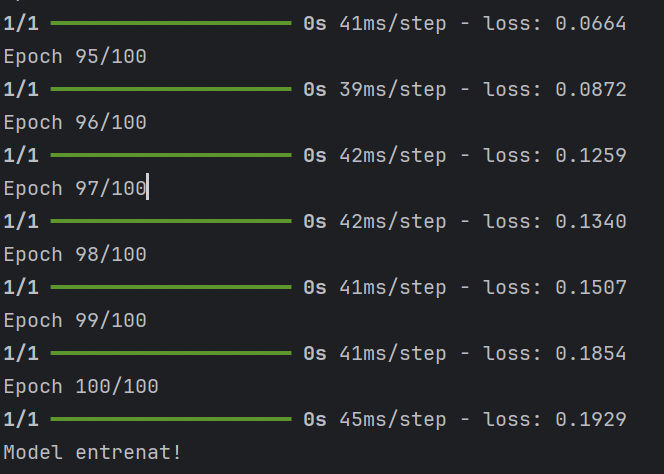
\includegraphics[width=0.5\textwidth]{./figures/11.png}
    \caption{Model entrenat}
\end{figure}


\begin{figure}[H]
    \centering
    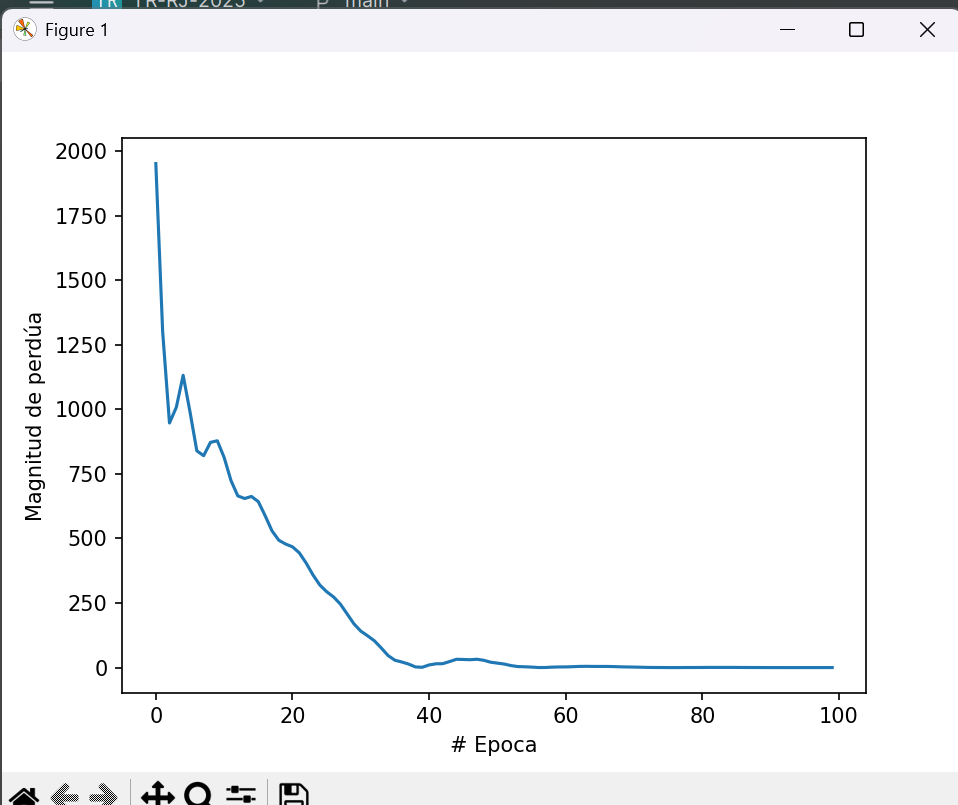
\includegraphics[width=0.5\textwidth]{./figures/12.png}
    \caption{Gràfica de la corba de pèrdua}
\end{figure}


\begin{figure}[H]
    \centering
    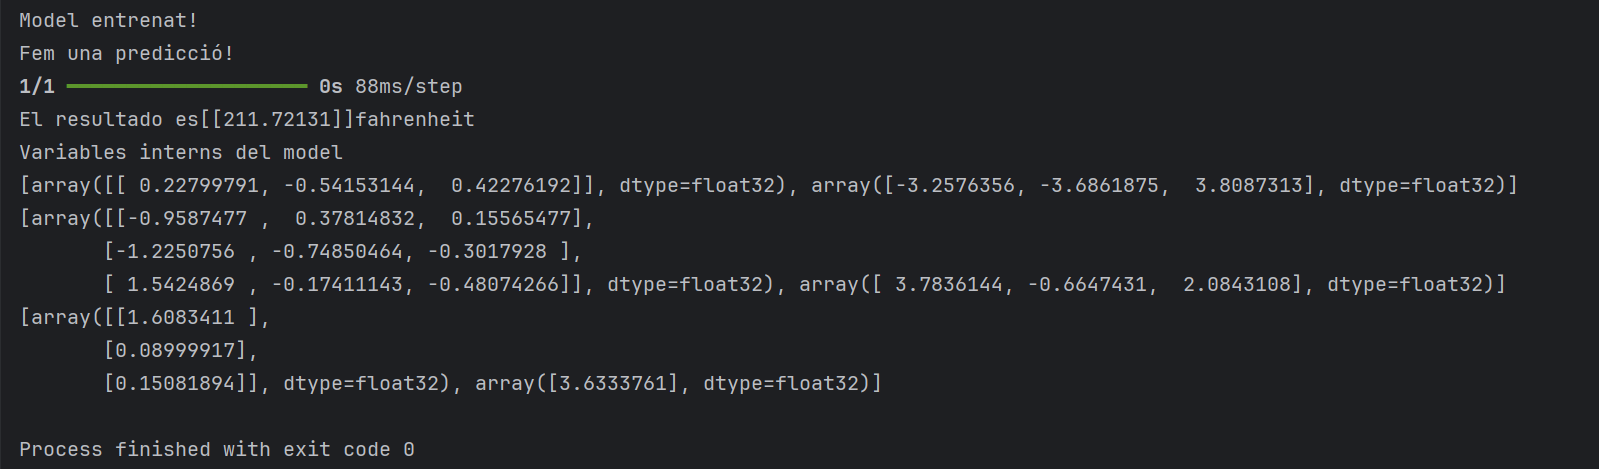
\includegraphics[width=0.5\textwidth]{./figures/13.png}
    \caption{El resultat de la predicció suposant que són 100 celcius el que ha de transformar i els baixos i pesos que ha utilizat la xarxa neuronal}
\end{figure}


Font: (\href{https://www.youtube.com/watch?v=iX_on3VxZzkhttps://www.youtube.com/watch?v=iX_on3VxZzk}{Xarxa neuronal amb Python})

\subsection{Predicció de les notes finals de matematiques }
Una vegada treballat amb la xarxa neuronal de celcius a fahrenheit, ja em trobo capacitat per fer la xarxa neuronal que ens haviem proposat, explicat en l'apartat \ref{sec:intr}

Igual que la xarxa neuronal de celcius a fahrenheit, començare amb la importació dels framework i biblioteques necessaries pel treball: \texttt{numpy}, \texttt{TensorFlow}, \texttt{matplotlib}, \texttt{MinMaxScaler}, \texttt{random} i \texttt{os}

\begin{itemize}
 \item \textbf{MinMaxScaler: } MinMaxScaler és una eina de la llibreria sklearn, la seva funció es normalitzar les dades i convertir els valors numerics dins del rang $[0,1]$, en que facilitarà molt la feina de la xarxa neuronal en entendre les relacions numerics.
 \item \textbf{random: } random és una llibreria bàsica del Python, aquest modul genera i selecciona nombres aleatoris.
 \item \textbf{os: } os també és una llibreria estandard del Python. el que ofereix aquest modul és per treballar amb el sistema operatiu.
\end{itemize}

\begin{figure}[H]
    \centering
    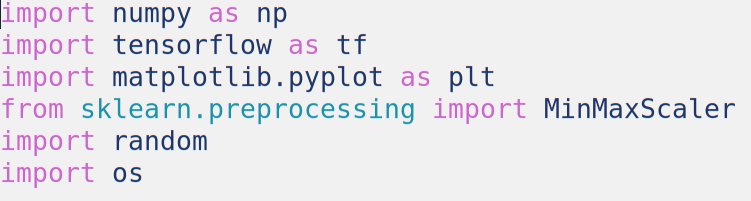
\includegraphics[width=0.5\textwidth]{./figures/21.png}
    \caption{Els biblioteques, llibreries i framework}
\end{figure}

A diferència de l’anterior xarxa, aquesta vegada he de fixar els resultats de la predicció per tal que les notes finals siguin més precises. Amb l’ajuda de la llibreria random pugues seleccionar qualsevol nombre aleatori que vulguessí, però per garantir la reproduïbilitat assignem la llavor (seed) amb el valor 42. Així, la xarxa neuronal sempre s’inicialitzarà amb els mateixos pesos i biaixos.

A continuació, controlo l’aleatorietat de les diferents llibreries que intervenen en el procés: \texttt{NumPy}, \texttt{TensorFlow}, \texttt{random} i, finalment, estableixo el valor del hash de Python amb la importació del mòdul \texttt{os}.

Control de l’aleatorietat:
\begin{itemize}
\item \textbf{Llavor:} \texttt{seed = 42}
\item \textbf{NumPy:} \texttt{np.random.seed(seed)}
\item \textbf{TensorFlow:} \texttt{tf.random.set\_seed(seed)}
\item \textbf{random:} \texttt{random.seed(seed)}
\item \textbf{Python:} \texttt{os.environ["PYTHONHASHSEED"] = str(seed)}
\end{itemize}

\begin{figure}[H]
    \centering
    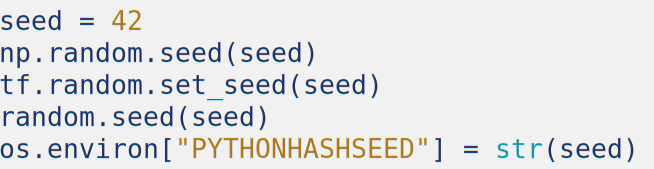
\includegraphics[width=0.5\textwidth]{./figures/22.png}
    \caption{Fixar els resultats de les prediccions}
\end{figure}


Una vegada d'haver fixat els pessos i biaixos, ja començo a emmagatzemar dades per l'entrenament de la xarxa neuronal. Llavors començo amb la de la entrada seguint d'aquest ordre tots sent la variable X:
 \begin{enumerate}
 \item Realització de deures
 \item Hores d'estudis (semanal)
 \item Hores de section
 \item Interès en la matèria
 \item Nota del segon trimestre
 \item Nota del tercer trimestre
 \item Nota final
 \end{enumerate}
 Posem \texttt{X = np.array([])} en que crea un llistat de dades, d'aquesta manera tan sol he de estar omplint les dades que he obtés del formulari que haviem creat, seguint una estructura de \texttt{[x1, x2, x3, x4, x5, x6]} i per ultim sempre acabo amb un \texttt{dtype=float} per indicar que el numero es un decimal.
 Després d'asssignar les dades d'entrades, arà toca constuir la de la sortida o també anomenat resultat/valor, que els considerare com a \texttt{y}, a diferencià del \texttt{X}, la sortida \texttt{y} només té una filera que representarà el valor que donarà cada filera dels \texttt{X} separades per una coma.
\begin{figure}[H]
    \centering
    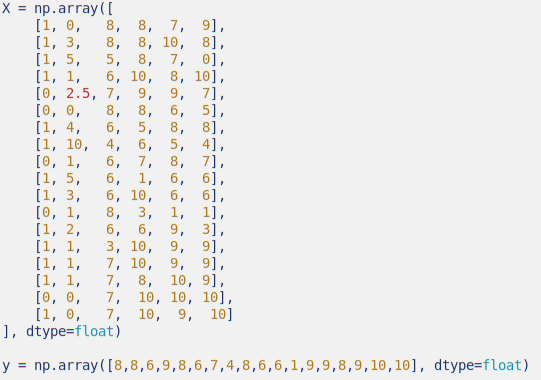
\includegraphics[width=0.5\textwidth]{./figures/23.png}
    \caption{magatzem de dades}
\end{figure}







\section{Xarxa Neuronal amb fulls de calculs}\label{sec:11}
En aquest apartat continuarem amb la xarxa neuranal de regressió però aquesta vegada utilizarem un full de calculs per fer-ho.
 L'estructura que utilitzarem per aquesta pràctica serà la del perceptró.

\begin{figure}[H]
    \centering
    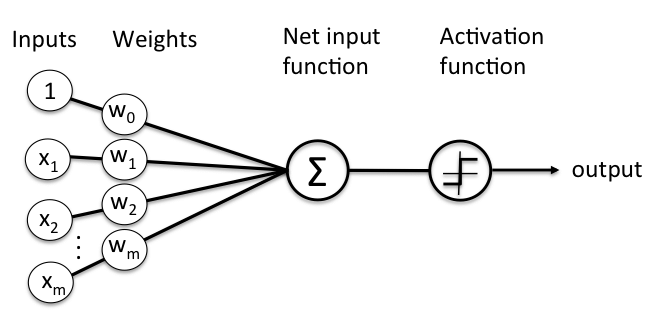
\includegraphics[width=0.5\textwidth]{./figures/perceptro.png}
    \caption{Estructura del perceptró}aaa
\end{figure}

Un cop sabem quina estructura utilitzarem, començarem la pràctica ordenant les dades de cada alumne del formulari en el full de càlculs

\begin{figure}[H]
    \centering
    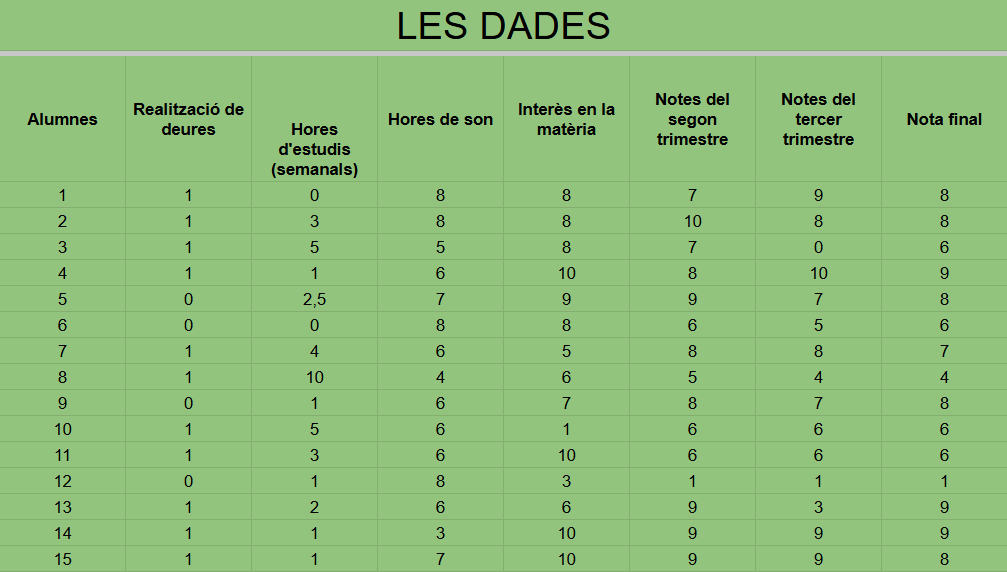
\includegraphics[width=0.5\textwidth]{./figures/Dades.png}
    \caption{Dades dels alumnes en el full de càlcul}
\end{figure}

Una vegada he ordenat tota la informació, he decidit representar els valors d'entrada d'una forma més senzilla d'entendre i curta, anomenantlos $xi$
\begin{itemize}
 \item \textbf {Realització de deures:} $x1$
 \item \textbf {Hores d'estudis:} $x2$
 \item \textbf {Hores de son:} $x3$
 \item \textbf {Interès en la matèria:} $x4$
 \item \textbf {Notes del segon trimestre:} $x5$
 \item \textbf {Notes del tercer trimestre:} $x6$
 \item \textbf {Nota final:}´ $y$
\end{itemize}

Aquestra representació queda així:

\begin{figure}[H]
    \centering
    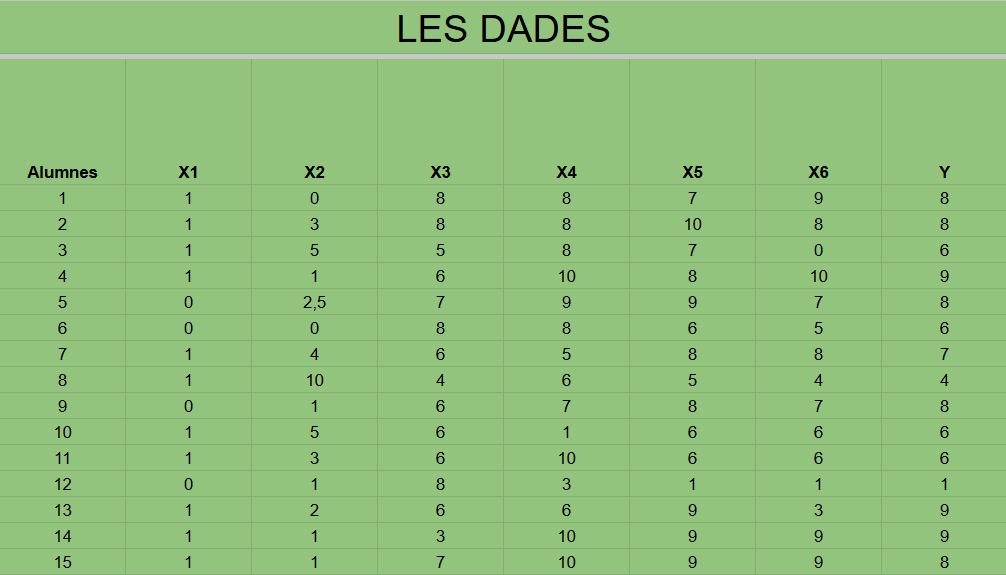
\includegraphics[width=0.5\textwidth]{./figures/Dades_resumides.png}
    \caption{Taula resumida}
\end{figure}

L'entrada de ``Realització de deures'' és una data binaria que nomès pot prendre valors 0 o 1.
\subsection{Normalització de dades}
Abans de continuar, és necessari explicar que és la normalització de dades.
La normalització de dades és una tècnica de procesament que consisteix en transformar dades de diferents escales a una escala comú, com per exemple del 0 al 1, aixó facilita la comparació i l'anàlisi de la xarxa neuronal i millora el seu rendiment. En el nostre cas, tenim dades binaries i dades ordinaries qe poden prendre qualsevol valor, aquest desequilibri afecta els càlculs posteriors si no es solucionen d'alguna manera.

Per aquesta raó, convertirem totes les dades en valors d'entre 0 i 1. Aquest procès implica calcular la miitjana de les dades i la desviació estàndar de cada variable. Per això utilitzant la fòrmula seguent:\\
$z = \frac{x - \mu}{\sigma}$\\

On:\\
$z$ És el valor normalitzat\\
$x$ És el valor original\\
$\mu$ És la mitjançan\\
$\sigma$ És la desviació estàndar\\

Aquests càlculs són fàcils d'obtenir amb les funcions que ens proporciona el full de càlcul.

\begin{figure}[H]
    \centering
    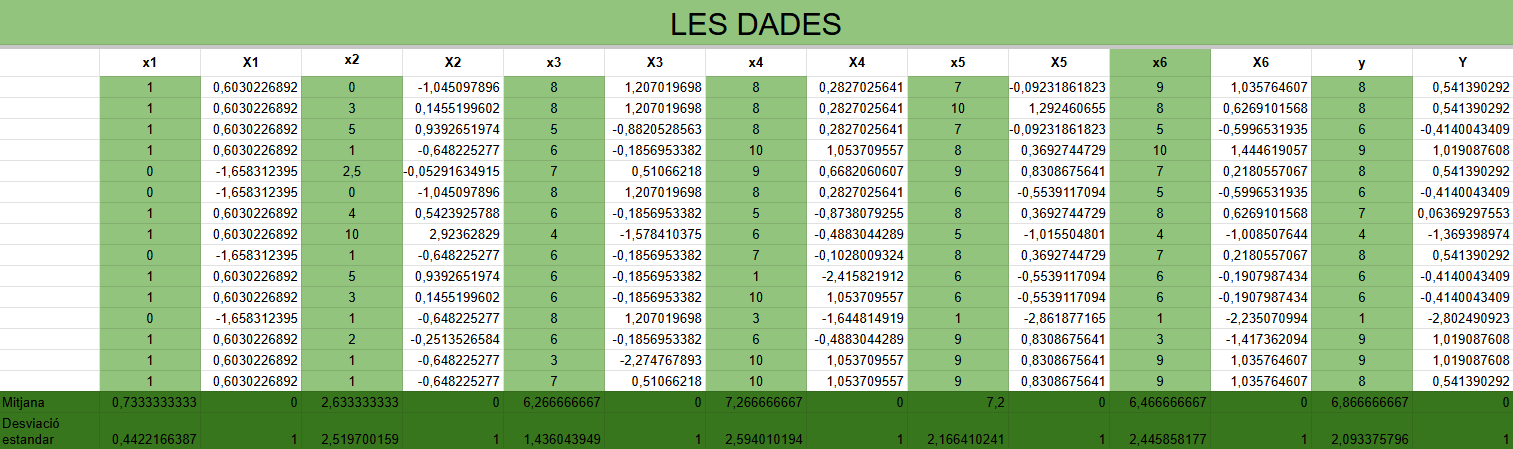
\includegraphics[width=0.5\textwidth]{./figures/Dades_normalitzades.png}
    \caption{Taula resumida}
\end{figure}

\subsection{Els paràmetres del model}
Ara que ja tenim totes les dades preparades, hem d'assignar a cada variable X el seu pes per determinar la seva importància en la predicció final. Al començament de l'entrenament, assignarem a tots els valors d'enrada el mateix pes, ja que es corregiran lentament durant l'entrenament.
També hem d'afegir el biaix,que és la constant que ajuda a millorar l'ajust de les prediccions.

\begin{figure}[H]
    \centering
    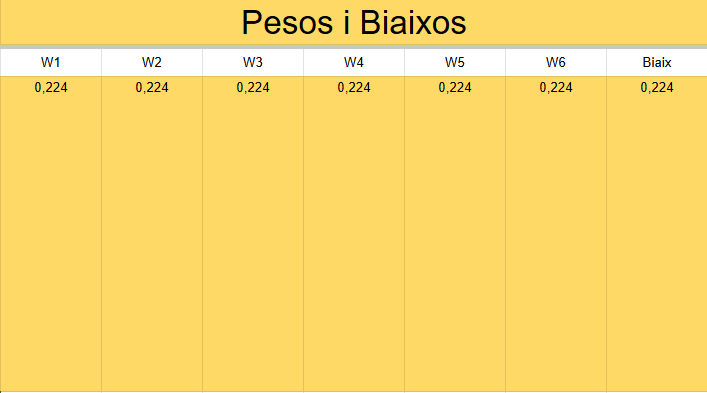
\includegraphics[width=0.5\textwidth]{./figures/Pesos.png}
    \caption{Taula dels pesos}
\end{figure}

En la figura 6.8 podem observar com ha quedat la taula després d'afegir els pesos als valors d'entrada, he afegit 6 columnes de pesos respecte a les 6 entrades i una columna més pel biaix.

\subsection{Funció d'error del model}
Fins ara, ja tenim les dades d'entrada normalitzades i els seus respectius pesos inicials assignats, per tant ja podem aplicar la fòrmula que s'utilitza en les xarxes neuronals per calcular la predicció temporal de la nota final. Hem de recordar que la fòrmula és:\\
\[
\sum w_i x_i + \text{biaix}
\] \\
Desprès d'aplicar la fòrmula, obtindrem la predicció de la nota final, tal com es veu en la figura 6.29.

\begin{figure}[H]
    \centering
    \includegraphics[width=0.5\textwidth]{./figures/Predicció.png}
    \caption{Prediccions del model}
 \end{figure}

Hem de recordar que els valors de la predicció són erronis, a que els pesos que hem assignat són aleatoris.

Per questa raò, el següent pas de la pràtcia és entrenar el nostre model per millorar els paràmetres. Per dur això, haurem d'aplicar un procès d'optimització per ajustar aquest paràmetres. En aquest cas utilitzarem l'algoritme gradient descendent, explicat anteriorment en l'apartat \ref{subsec:gradient}.

Començarem afegint més columnes en el nostre full en la nostra taula. Si restem els valors de la predicció ($Y$) amb els valors reals ($y$) obtindrem la diferència entre la nota dels alumnes i les notes predictives.

\begin{figure}[H]
    \centering
    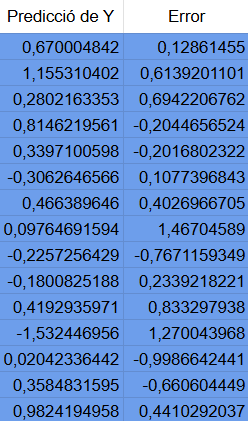
\includegraphics[width=0.5\textwidth]{./figures/Errors.png}
    \caption{Erros de la predicció}
\end{figure}

Es pot veure en la imatge 6.30 dues columnes adicionals, la columna ``error'' emmagatzema els errors del model i l'altre conté els mateixos errors pero en valor absolut, es a dir, que tots els valors estan en positiu, d'aquesta manera serà més fàcil apreciar la diferència dels errors en les prediccions i els càlculs dels paràmetres.

Després de crear aqeustes taules, calcularem la mitjana dels valors que estan en la taula dels errors en positiu, el resultat d'aquesta mitjana ens ajudarà a orientar-nos i determinar si en cada iteració l'error està augmentant o disminuint, quan més baix sigui aquest valor, la predicció serà més precisa.
\subsection{Canvis dels paràmetres}
Un cop tenim la funció d'error de la primera predicció, el pas següent és entrenar el model per ajustar els valors dels pesos i del biaix adequadament perquè les següents prediccions siguin més precises.
Per aconseguir aixó, hem de tindre en compte les dades seguents: Quan la diferència de $Y$ respecte a $y$ és més gran, més luny estaran els pesos dels seus valors ideals. Per tant hem de trobar la forma de calcular de forma correcta els pesos respecte de la diferència dels valors de l predicció.

Gràcies a la fòrmula de la xarxa neuronal sabem que si el valor d'entrada ($X$) és petit, el seu pes ($W$) també ho serà, ja que aquests es multipliquen. Per tant hem de tindre en compte dues coses: La diferènccia de la predicció final ($Y$) i del valor real ($y$) i el valor d'entrada ($X$) respecte al seu pes ($W$). Per tant fòrmula que utilitzarem per calcular els canvis dels paràmetres serà:\\
$\Delta W = (Y_{\text{original}} - Y_{\text{predicción}}) \times X$\\
Aquesta fòrmula serà la que ens ajudarà a ajustar els paràmetres per tal de que la predicció sigui cada cop més precisa. Aplicant aquesta fòrmula a cada una de les dades, obtindrem 7 columnes més.

\begin{figure}[H]
    \centering
    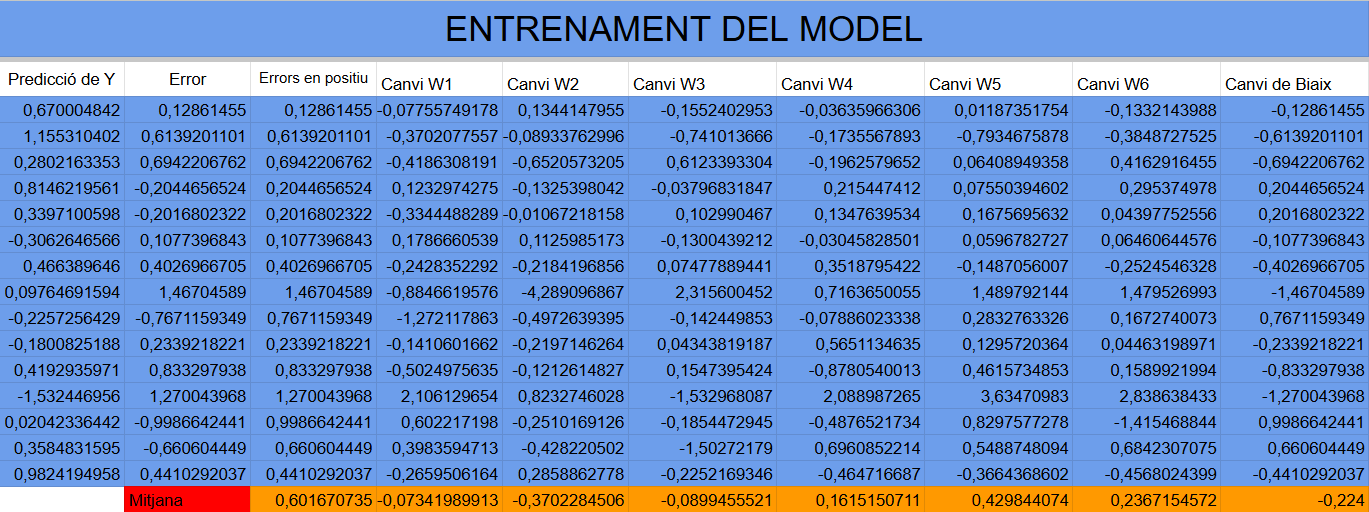
\includegraphics[width=0.5\textwidth]{./figures/Canvis.png}
    \caption{Canvis en els paràmetres}
\end{figure}

En la figura 6.31 es por veure com han quedat aquestes taules, els cnvis del biaix es calculen amb la mateixa fòrmula que els pesos, pero sense restar-li cap entrada, ja que actúa com una entrada constant.

Ara és necesari calcular la mitjana dels cavis dels pesos, les mitjanes obtingudes a partir dels canvis seran uns dels valors que utilitzarem per ajustar els paràmetres.

\subsection{La taxa d'aprenentatge}
Avans de començar a entrenar el model, hem de parlar d'una variable molt important, que és la taxa d'aprenentatge. Auesta taxa és un paràmetre ue ajsta l'ample dels pasos que fem per actualitzar els pesos i el biaix del model, com vam explicar a l'apartat \ref{subsec:gradient}, el valor d'auesta taxa no pot ser molt gran perquè si no no es podria trobar el punt de convergència, ni molt petit perquè relentitzaria la xarxa.

Normalment la el valor de la taxa d'aprenentatge és 1, però de vegades auest valor és molt gran i augmentaria l'error del model, si això pasa hauriem de reduir el seu valor progressivament fins un punt on l'error de la xarxa disminueixi significativament.

Finalment, per trobar el valor final dels canvis ajustats dels paràmetres haurem de multiplicar a mitjana dels canvis dels pesos per la taxa d'aprenentatge.
\subsection{Èpoques d'entrenament}
Ja podem començar a entrenar el model, ho farem copiant la mateixa taula que tenim a sota, com es veu en la figura 6.13.

\begin{figure}[H]
    \centering
    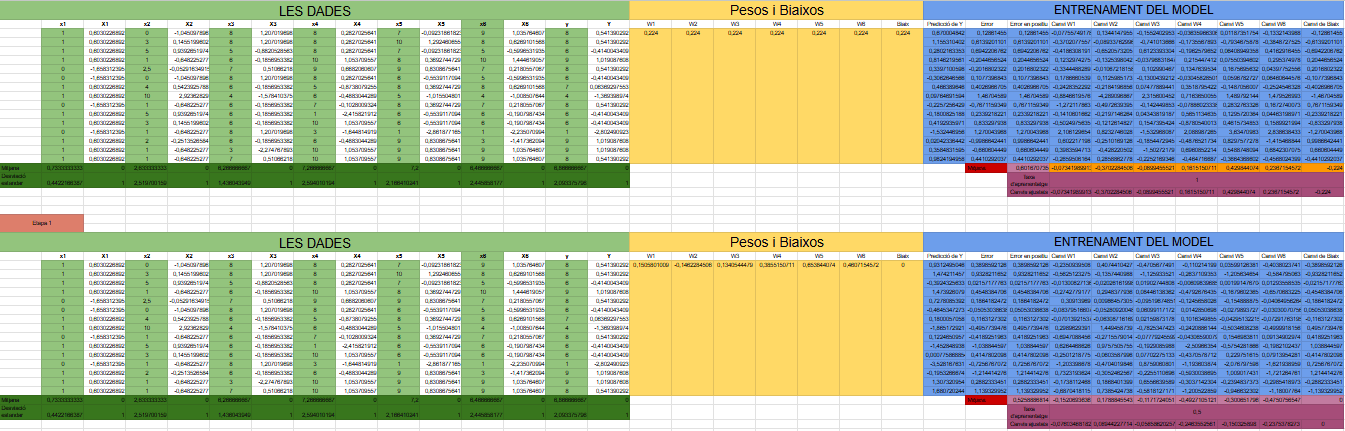
\includegraphics[width=0.5\textwidth]{./figures/Etapa_1.png}
    \caption{Èpoques d'entrenament}
\end{figure}

Cada època d'entrenament seria com si fos una iteració, podem veure que els paràmetres de la primera època han canviat respecte de la primera taula, que li anomenarem època 0, on aquests pràmetres eren inicialment aleatoris, el valor del primer pes de l'època 1 ($W1$) es calcula sumant el pes de la època 0 pel valor del canvi ajustat.
Per saber si el model ha millorat, la millor forma de comprobar-ho és fixant-se en la taula dels errors en positiu. Podem veure que aquest valor ha disminuit respecte a l'epoca anterior, això significa que esttà millorant.
A partir d'ara hem de fer ho mateix repetidament fins que el canvi de l'error entre les èpoques siguin molt petits, quan pasi això significarà que estem pràcticament en el punt de convergència, i és important anant ajustant la taxa d'aprenentatge.
\subsection{Resultats}
En aquest cas, ha calgut de 8 etàpes per arribar al punt de convergència. He organitzat els valors de l'error de cada època en una gràfica per que sigui més fàcil visualitzar els canvis

\begin{figure}[H]
    \centering
    \includegraphics[width=0.5\textwidth]{./figures/Gràfica_error.png}
    \caption{Gràfica dels valors d'error en cada època}
\end{figure}

En la figura d'adalt podem apreciar que l'error ha disminuit dràsticament entre l'època 0 fins l'època 3, pero després de la tercera època l'error pràcticament no s'ha mogut, vaig ajustar la taxa d'aprenentatge moltes vegades pero l'error encara baixava molt lentament, fins que vaig arribar a l'etapa 8 on l'error casi no baixava. Això vol dir que el model no ppodia ajustar més els pesos i que ja havia après.

\section{Comparació entre una xarxa neurnal creada per un llenguatge de programació netre una de fulls de calculs}

\section{Xarxa Neuronal amb un cas real}\label{sec:12}
